\chapter{Techniques}
\label{Chapter4}
\lhead{Chapter 4. \emph{Codes}}

Throughout this thesis my goals were to identify SLSNe in a number of surveys. I have approached this problem using a number of tools and techniques, each playing an important role in achieving this goal. The aim of this chapter is to provide and overview of the methods used in this work as well as their evolution over time. In the early parts of this thesis, I used an approached based on modelling of SLSNe using the popular spin-down of a magnetar model \sref{sec:SLAP}. I begin by describing the model and the improvements I have introduces in order to better model the UV region of the SLSN SED. I also describe the fitting routines used in the modelling of SLSNe as well as throughtout the entire thesis. Although, this technique was successful in identifying a new SLSN in the SNLS, it was not able to fully capture the diversity of the SLSN sample that was emerging in the DES spectroscopic dataset. As a solution to this problem, I followed a popular route of applying the state-of-the-art artifficial inteligence (AI) technqiues to automate the classification process using a machine learning approach. The second part of this chapter describes the preparatory work undertaken to build the tools and the training sample required for such study in \cref{Chapter5}.

The use of ML moved the focus of this work away from understanding the parameter space of the SLSNe model, or the choice of cuts needed to define them. Instead I have focused on simulating DES and its tranients. This includes SNIa, both hydrogen poor and rich CCSNe, SLSNe, AGNs as well as random noise spikes which are the main source of contamination in the data. The models of SNIa are mature and ready to be deployed in this work thanks to being used as cosmological probes for over two decades. Simulations of CCSNe, however, have not sparked an equal amount of enthusiasm amonst the SN community until recently, hence became a one of the key subjects of this thesis. CCSN are usually faster and fainter than SNIa resulting is a significantly smaller sample of well observed objects. The number of objects with a high quality spectroscopic follow-up are also much lower compare to SNIa. In recent years, the interest in modelling these objects has increased dramatically with large projects, such as LSST, requiring samples of fake transients in order to inform the design of their observing strategies. In this chapter, I describe our approach to creating a new spectroscopic set of CCSN templates as well as simulating them in a number of surveys. This project was build to provide a sample of stripped-envelope CCSNe as part of the LSST photometric lightcurves classification challenge. However, later I have applied it to DES in order to produce both a samples of hydrogen rich as well as poor CCSNe.

The last, but perhaps the most important, technique descrined in this chapter is Gaussian Processing (GP). DES, similarly to other transient surveys, was not observed on regular cadance. However, most machine learning techniques require evenly samples data. I used Gaussian Processes as a method for interpolating the light curves independantly of any model which could be used to simualate the objects. GPs are based only on the uncertainties associated with the data and produce a confidence regions for the underlying light curves. This is key in solving the overfitting problem when working with artificial training sample within Machine Learning.

This chapter is divided in the following way; I begin by describing the methods behind the modelling of SLSNe using the magnetar model as well some some basic extensions in conjunction with SED templates. Following this, I discuss the search for SLSNe as well as their pre-peak `bumps' and other rapidly evolving transients in DES. Next, I describe the method of Gaussian Processing light curves as a model-independant approach to interpolating our data. Finally, I describe the techniques behind the modelling and simulating of CCSN in the context of DES.

\section{Modeling SLSN Light Curves} \label{sec:SLAP}
Throughout this thesis the modelling of SLSNe light curves plays a pivotal role. The measurement of the rate of SLSNe presented in \cref{Chapter3} as well as the search for SLSNe in DES described in \cref{Chapter5,Chapter6} uses a definition of SLSNe based on the spin-down of the magnetar model. The choice of the magnetar model as our main tool came after a simpler model, describing SLSNe using and linearly expanding and cooling photosphere, was tested but eventually rejected in favour of the magnetar model. I introduce this basic model, including its drawbacks, before I describe the magnetar model along with the improvements it brings to the modelling of SLSNe.

When modelling light curves of SLSNe there are two independant, but equally important, areas that contribute to the accuracy of the model: the spectral energy distribution (SED) of the SN, and its evolution with time. The need to model the SED of a SN could be avoided if we used an approach which purely relied on the bolometric lightcurves as opposed to multi-band observations. From the software implementation point-of-view these models are easier to use, and are common in the literature \citep{Inserra2013,Papadopuplus2014,Nicholl14}. However, they do not consider the colour, along with its evolution, of a SN which provides a very powerful tool for further constraints the properties of the SNe. It has been previously shown \citep{2011ApJ...743..114C,2013ApJ...779...98H,2015MNRAS.449.1215P,2014ApJ...797...24V} that the SLSN SED can be accurately approximated, in the visible spectrum, by a slowly evolving (nearly) perfect blackbody with an addition of their characteristic broad lines of O\,II. However, this approximation breaks down in the near UV due to the prominant broad absorption features which can be attributed to Mg\,II, Fe\,III, C\,II, Co\,III, Si\,III and Ti\,III \citep[see][for line identifications]{Mazalli2016}.

\subsection{Improving the blackbody approximation}
In order to improve the reliability of SLSN SED modelling, I propose a method of improving the blackbody approximation by superimposing absorption template onto the simple blackbody SED. In order to derive these template, I use a method similar to tht of  \citet{2014ApJ...797...24V} where I fit the Planck function to several featureless, 50$\AA$ wide regions of the spectrum in order to measure the underlined blackbody continuum in the SED, as shown in figure \ref{fig:specTemplate}. The resulting fits show that the absorption relative to the blackbody is low in the regions of $\lambda>3000\AA$, and increases drastically in the bluer regions of the spectrum.

The time evolution of the spectra appears to be weak in comparison to other SNe, making it possible to approximate the SED at any epoch using the Planck function, where the temperature evolves with time, and a single absorption template is used. The absorption is calculated as a ratio of the observed flux to the continuum blackbody fit. The number of SLSNe with good UV coverage remains small, with only the spectra of iPTF13ajg \citep{2014ApJ...797...24V}, SCP06F6 \citep{2009ApJ...690.1358B} and SNLS-06D4eu \citep{2013ApJ...779...98H} providing sufficient data until the discovery of Gaia[CITE AND INSERT NUMBERS]. Do due to the observer-frame coverage of their respective spectra, our spectral templates cover a rest-frame wavelength range of 1620--3320\,\AA\ (SNLS-06D4eu), 1800--3800\,\AA\ (SCP06F6) and 1800--5250\,\AA\ (iPTF13ajg). [PERHAPS REMOVE THIS TO MAKE IT LESS HARD ON MYSELF]
\begin{figure}
\centering
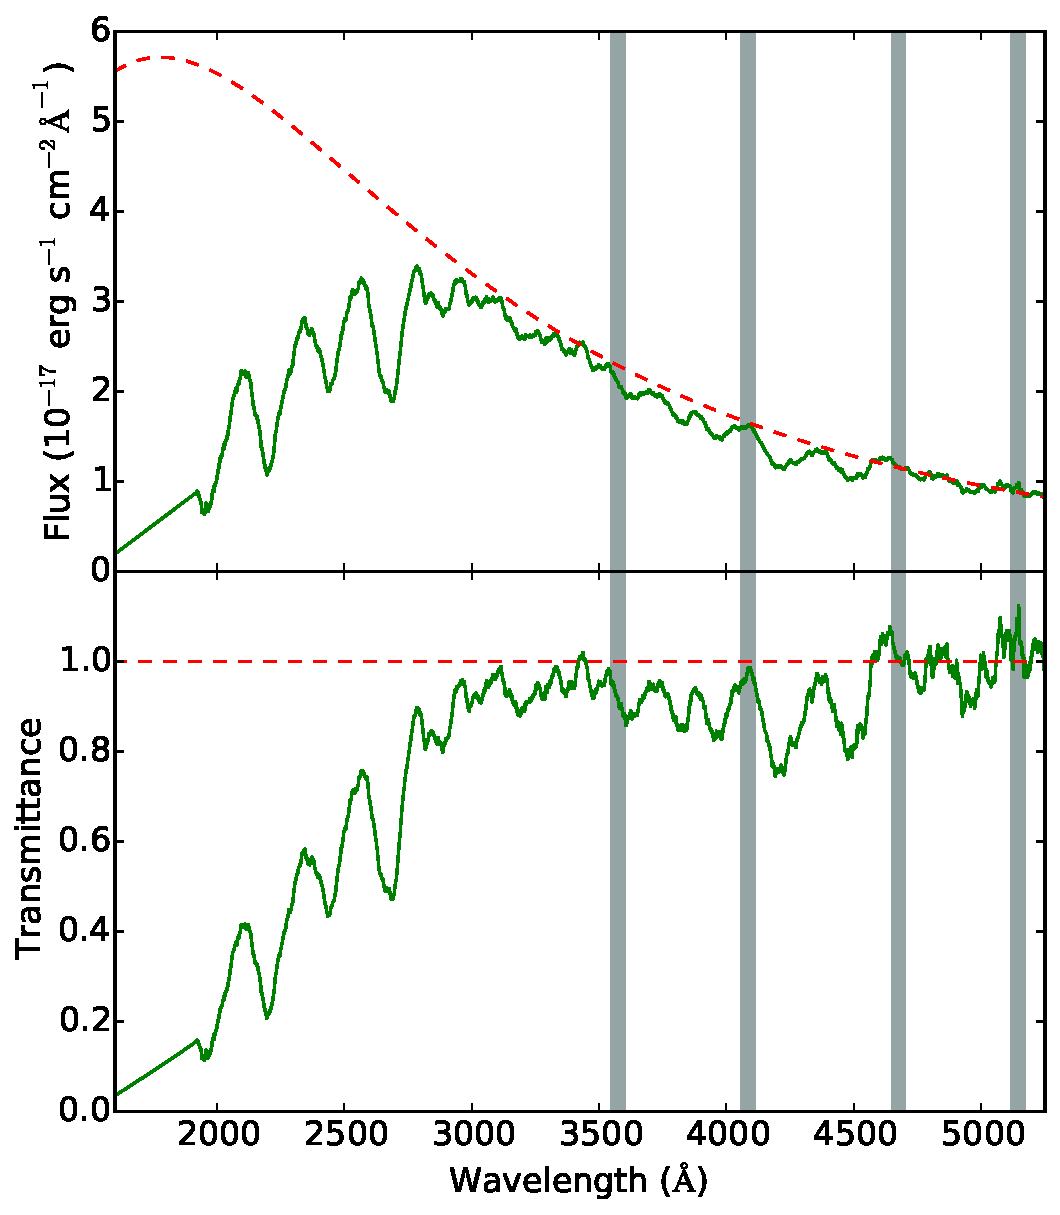
\includegraphics[width=\textwidth]{Figures/Chapter4/specTemplate}
\caption{iPTF13ajg is fitted with the Planck function. The spectrum of iPTF13ajg (green) can shows a good agreement with the blackbody (red) at $\lambda>3000\AA$. At lower wavelengths a strong deviation from the model is observed, highlighting the need for a correction to the model. The ratio between the observed spectrum and the continuum give a measure of the absorption strength as a function of wavelength and can be used in modelling the SLSN SED.}
\label{fig:specTemplate}
\end{figure}

\subsection{Modelling the SED evolution}
The ability to describe the SEDs of SLSNe as blackbodies greatly simplies the
modelling of its evoution. A model is only required to provide the thermal and radial evolution of the photoshere, therefore removing the need for complex modelling such as radiative transfer or hydrodynamic simulations.

\subsubsection{Fireball model}
Perhaps the simplest approach to modelling the SED evolution is to assume that the SN, with an initial radius R$_{0}$ and initial temperature T$_{0}$ expands at a constant rate while cooling down also at a current rate as seen in \eref{eq:Howell}
\begin{align}
\label{eq:Howell}
R(t) &= R_0 + \dot{R}t &&\\
T(t) &= T_0 - \dot{T}t &&
\end{align}
\noindent While this model is not physical motivated, \citet{Howell2013} showed that it provides a good, first-order approximation to the light-curves of SLSNe. Due to its simplicity, the model appeared as an attractive prospect for the modelling of SLSN SEDs. However, our testing showed that while it produces a good fit to a SLSN around the maximum light (<+30days) it is not able to capture the slow evolution in the tale of the light curve as seen in \fref{fig:BB_Mag} making in infavarable in comparison with the more complex magnetar model.

\begin{figure}
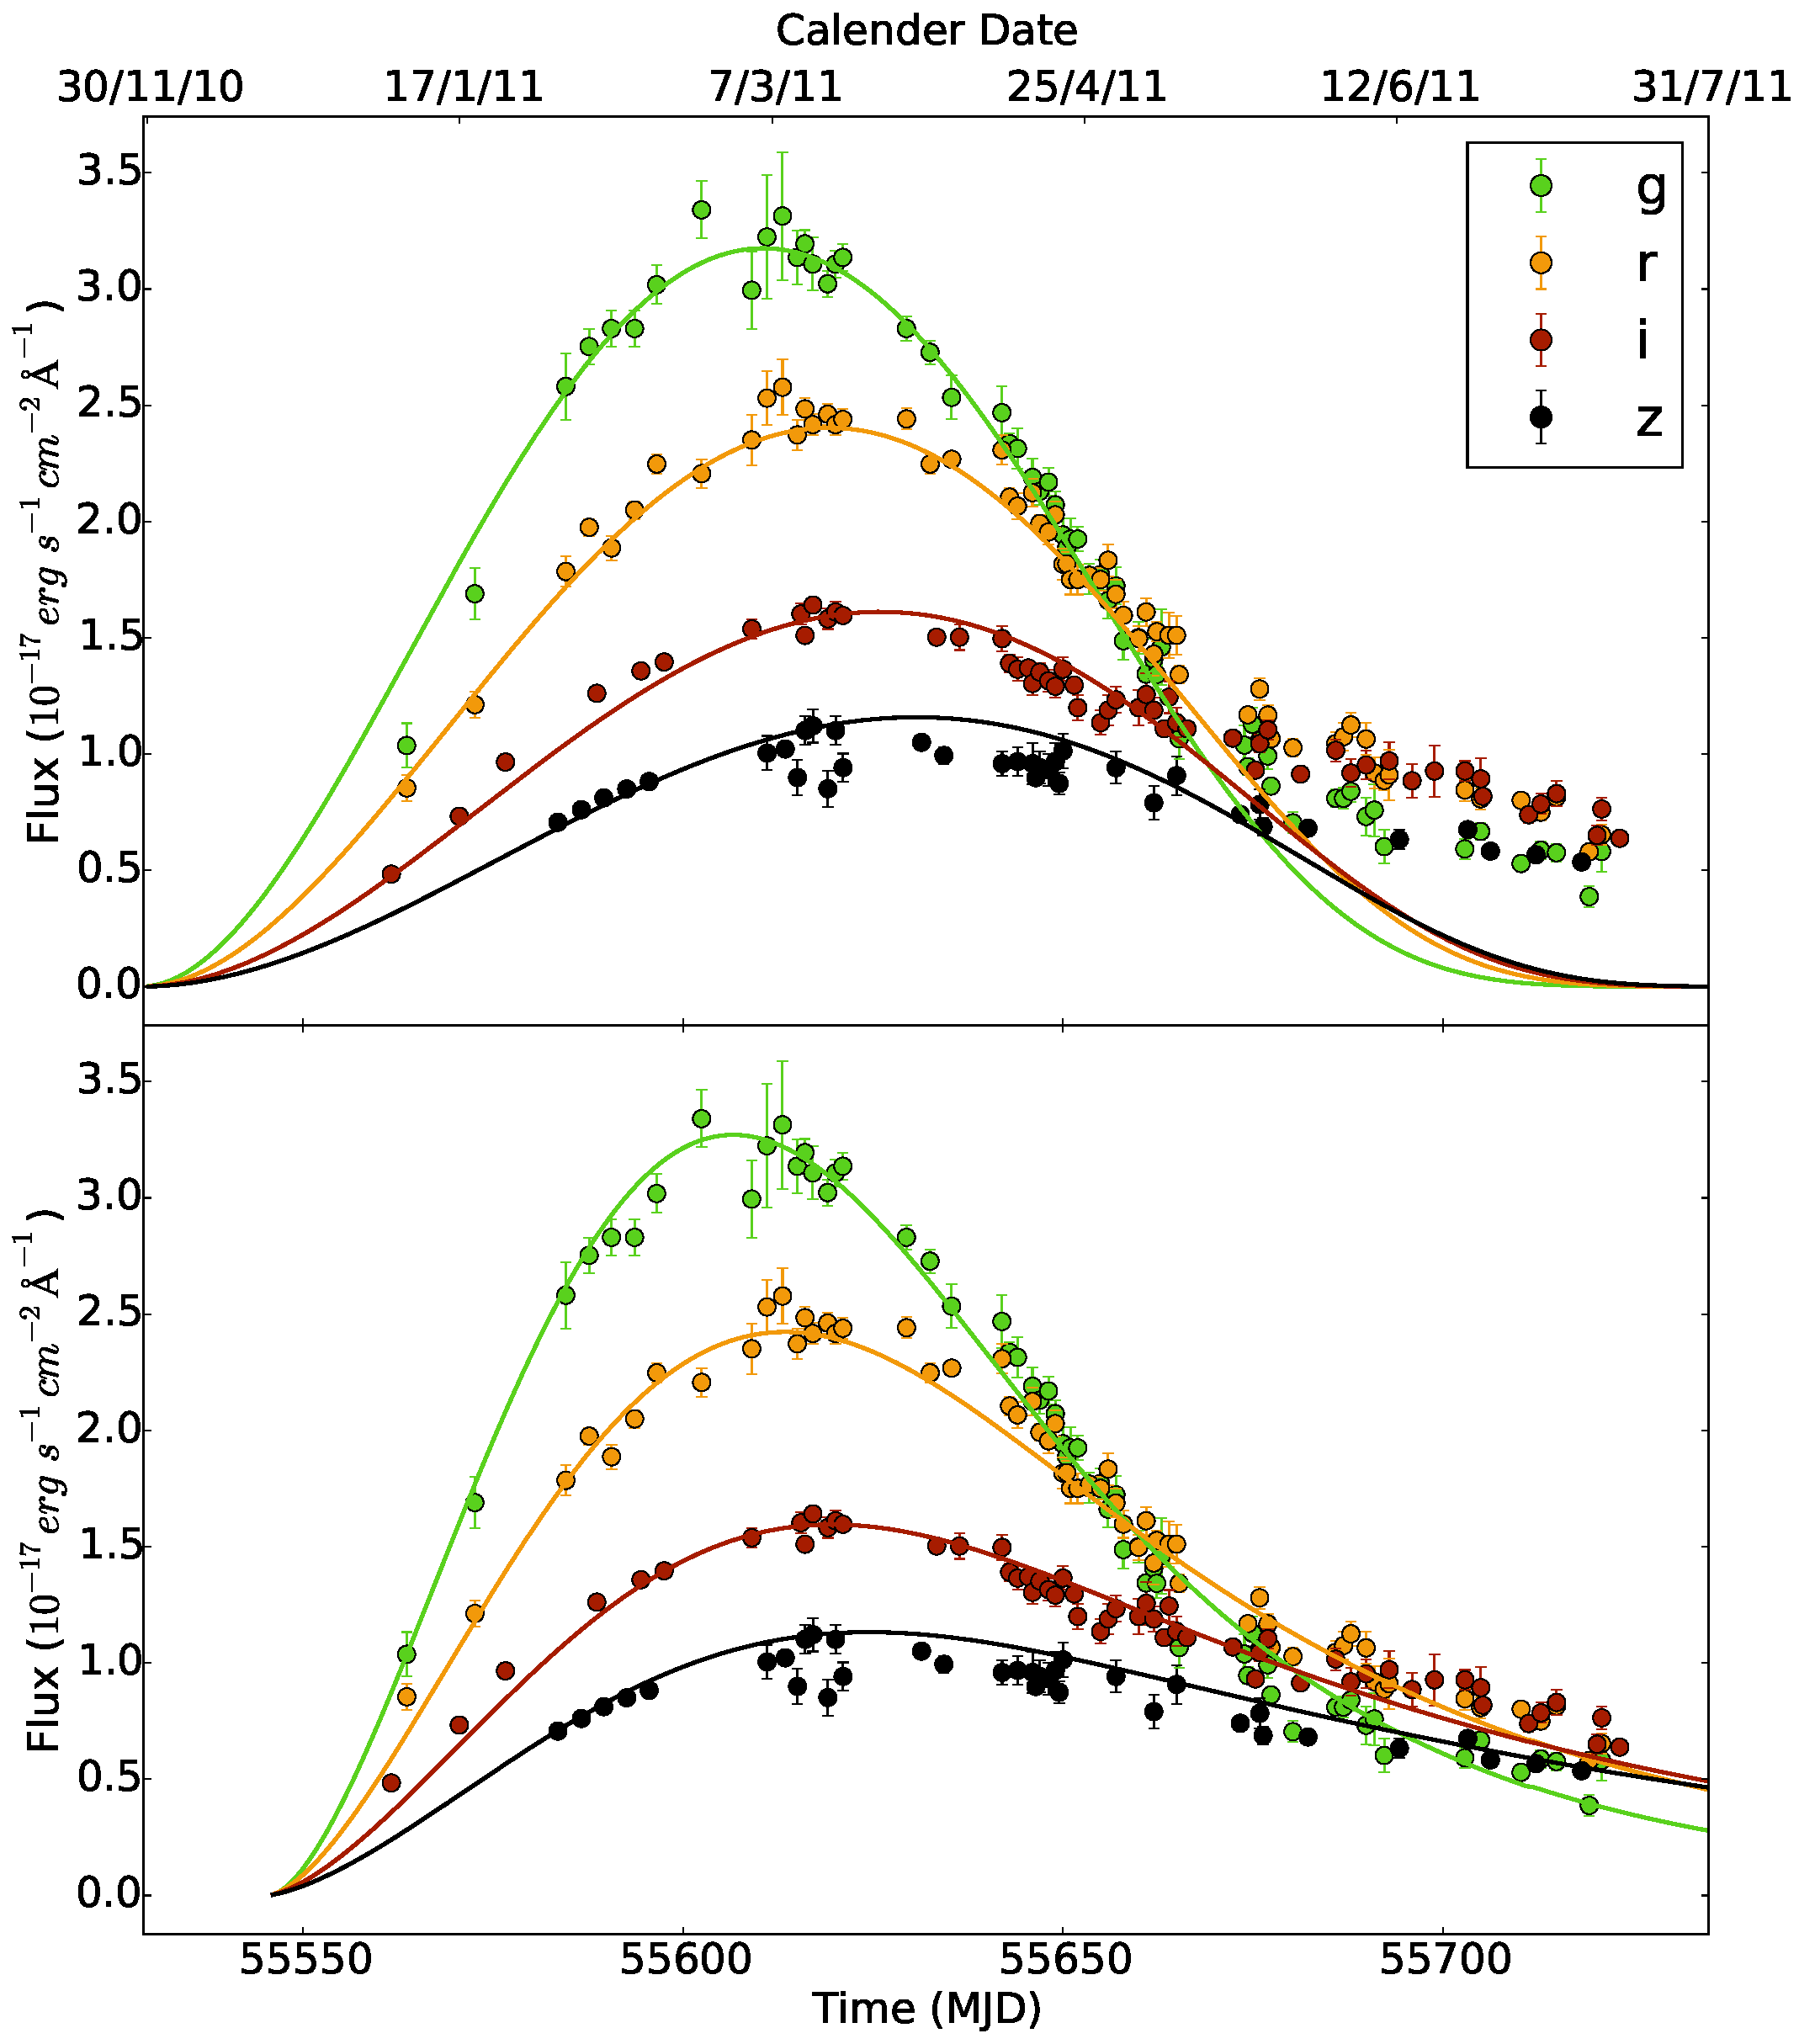
\includegraphics[width=\textwidth]{Figures/Chapter4/BB_Mag_comp}
\caption{The SLSN PS1-11ap $griz$ light curve \citep{2014MNRAS.437..656M} compared to two models describing its photometric evolution. In the upper panel, the model is a simple expanding and cooling blackbody fitted to data around maximum light only, and in the lower panel the model is our `absorbed' magnetar model fitted to the entire light curve. In the case of the magnetar model, the spectrum of SNLS-06D4eu \citep{2013ApJ...779...98H} has been used as an absorption template in the modelling of the SED \sref[see]{sec:KCorrection}). Note that while both models can produce reasonable fits around the peak of the light cuve, the black body model is not able to reproduce the characteristic late-time behaviour of SLSNe. Light curve phases are measured with respect to peak brightness in the rest-frame \textit{u}-band as predicted by our magnetar model fit.}
\label{fig:BB_Mag}
\end{figure}

\subsubsection{Magnetar model}
\label{sec:Magnetar}
To fully capture the evolution of the SED with time we must employ a model for an engine that provides the late time energy deposition needed to explain the photospheric velocity and temperature observed in SLSNe. While still a matter of active debate in literature, in recent years the birth and spin-down of a magnetar model has appeared as the strongest candidate to explain these extremely luminous events \citep{2013ApJ...770..128I,2013Natur.502..346N}. In this model, SLSNe begin as CCSN with a magnetar, a rapidly rotating, highly magnetised neutron star, born at its core. As the magnetar spins down due to the interactions with its environment, it dissipates its energy in the form of high energy radiation that is then captured by the expanding ejecta and thermalised to produce the observed blackbody SED \citep{2010ApJ...717..245K,2010ApJ...719L.204W,2012MNRAS.426L..76D}.

I follow the method from \citet{2013ApJ...770..128I}, based on the Arnett law for the energy diffusion through SN ejecta \citep{Arnett1982}, and the energy radiated by the central engine from \citet{Bildsten2013,Wosley2012}. In order to model the bolometric luminosity, $L$, of a SLSN as a function of time, $t$, we use equation \ref{Eq:MagnetarLum}:
\begin{equation}
L(t) = 4.9\times 10^{46}\,e^{ -(t / \tau_\mathrm{m})^2 }\delta(t) \int_{0}^{t} \frac{2t'}{\tau_\mathrm{m}^2}\,e^{(t'/\tau_\mathrm{m})^2}\,\frac{B_{14}^{2}\,P_{\mathrm{ms}}^{-4}}{\left(1+t'/\tau_\mathrm{p}\right)^2} dt',
\label{Eq:MagnetarLum}
\end{equation}
\begin{equation}
\label{Eq:SDPeriod}
\tau_{p} = 4.7B_{14}^{-2}P_{ms}^{2}days
\end{equation}
\noindent where $\tau_\mathrm{m}$ is the diffusion timescale, $B_{14}$ is the neutron star magnetic field in units of $10^{14}$\,G, $P_{\mathrm{ms}}$ is the magnetar spin period in ms, $\delta(t)$ is the deposition function or trapping coefficient, and $\tau_\mathrm{p}$ is the magnetar spin-down timescale, is defined in \eref{Eq:SDPeriod}, inferred from $B_{14}$ and $P_{\mathrm{ms}}$.

Physically $\tau_M$ is proportional to the ejecta mass($M_{ej}$) which is sometimes chosen as the fit parameter instead. The two parameters can be interconvert using equation \ref{Eq:Mej}, where $E$ is the explosion energy and $\kappa$ the opacity of ejecta.
\begin{equation}
\label{Eq:Mej}
M_{ej} = (\frac{\tau_{M}}{10days})^{4/3}(\frac{\kappa}{0.1cm^2g^{-1}})^{-2/3}(\frac{E_k}{10^{51}erg})^{1/3}M_{\odot}
\end{equation}
\noindent It has been shown \citep{2013ApJ...770..128I,2014ApJ...796...87I,2015MNRAS.452.3869N,2015MNRAS.449.1215P} that the opacity and the explosion energy parameters have only a weak affect the quality of fitting and have therefore been fixed as $\kappa = 0.1cm^2g^{-1}$ and $E = 10^{51}$erg respectively.

The velocity of the ejecta, $v_{core}$ are assumed to be constant and value can be found using the inferred mass of the ejecta, $M_{ej}$ and its kinetic energy, $E_{mag}$ (\eref{Eq:vcore}), which in turn depends on the explosion energy and the energy released by the spin down of the magnetar, shown in \eref{Eq:Emag}:
\begin{align}
\label{Eq:Emag}
E_{mag} = 4.9\times10^{46} B^2 P^{-4} \tau_{P}  \text{ erg} \\
E_k = 10^{51} + 0.5 \times E_{mag} \text{ erg}\\
\label{Eq:vcore}
v_{core} =  \sqrt{\frac{10 E_{k}}{3 M_{ej}}} \text{ cm s}^{-1}
\end{align}

\paragraph{Trapping coofficient}
The trapping coefficient, $\delta(t)$, is defined as the fraction of the high-energy radiation produced by the central engine that gets trapped, and subsequently reproduced as visible light, by the ejecta. It is often assumed in the literature that the trapping coofficient is time-independent and close to unity, implying the full trapping of radiated by the supernova ejecta \citep{2013ApJ...770..128I,2015MNRAS.449.1215P,2015MNRAS.452.3869N}. In this work I use a correction introduced by \cite{2015ApJ...799..107W} with a time-dependent trapping coefficient:
\begin{equation}
\delta(t) = 1 - \exp\left({-\frac{9\kappa \mathrm{M}_{\mathrm{ej}}^{2}}{40\pi  E_k} t^{-2}} \right),
\label{Eq:Wang}
\end{equation}
\noindent where $\mathrm{M}_{\mathrm{ej}}$ is the ejecta mass, $E_k$ is the explosion energy, and $\kappa$ is the opacity. $\mathrm{M}_{\mathrm{ej}}$ is proportional to $\tau_\mathrm{m}$, $E_k$ and $\kappa$ \citep{2013ApJ...770..128I}. We again fix the explosion energy to be $E_k = 10^{51}$\,erg and the opacity as $\kappa =0.1$\,cm$^2$g$^{-1}$.

Using this time-dependent trapping coefficient improves the late-time fit to the light curve. For a typical SLSN we calculate $\delta \simeq 1$ up to 75 days post explosion. However, as the ejecta opacity to high energy photons decreases with time we find $\delta \simeq 0.8$ at 150 days post explosion, emphasising the importance of this correction in the late time light curves.

\paragraph{Deriving Radius and Temperature}
In its simplest form, the magnetar model only predicts the total radiated energy of the SN and does not make any predictions about the SED of the object. It is therefore most commonly used with bolometric light curves, synthesised from the photometry. \citet{2013ApJ...770..128I}, however, shows that it is possible to predict the photospheric radius of a SN based on this model deriving the following equations:
\begin{equation}
\label{Eq:R19}
R(t) = r_{core}(t) \left(\frac{\alpha - 1}{\tau_{core}(t)}\right)^\frac{1}{1 - \alpha}
\end{equation}
\noindent while the radius of the photosphere exceeds that of the core ejecta, and;
\ref{Eq:R20}.
\begin{equation}
\label{Eq:R20}
R(t) = r_{core}(t) - \frac{1 - \frac{\tau_{core}(t)}{\alpha - 1}}{\kappa \rho_{core}(t)}
\end{equation}
\noindent when the photosphere recedes into the core. $r_{core}(t)$, $\rho_{core}(t)=$ and $\tau_{core}(t)$ are defined as follows:
\begin{align}
r_{core}(t) = v_{core}  t \\
\rho_{core}(t)= \frac{3 M_{ej}}{4  \pi  r_{core}^3(t)}\\
\tau_{core}(t) = \kappa  \rho_{core}(t) v_{core} t
\end{align}

Combining this with the total luminosity and assuming that the object radiates as a uniform, spherical blackbody gives us the photospheric temperature. This can be injected into the Planck law to give an approximation for the SED of a SLSN. This method allows for the magnetar model to be fit directly to the multi-band photometry without the need to produce the pseudo-bolometric light curves. We combine this with the absorption templates to produce a model of the SLSN spectral evolution as a function of time.

\subsection{SLAP}
Upon establishing an approach for modelling SLSNe it was important to encapulate it in a software package capable of performing under a number of situations. In this thesis the magnetar model was used in fitting the light curves of both known SLSNe and a variaty of transients, the majority of which could not be well approximated using this model. We have also used it in simulating SLSN in SNLS as well as producing an artificial training sample for the DES machine learning study of SLSNe.

The code was required to satisfy the following requirements:
\begin{itemize}
  \item Fit the magnetar model to all literature SLSNe and estimate their parameters.
  \item Perform a succesful fit to any light curve and return an output, regardless of whether it is physical.
  \item Move the object to any redshift within the range of SNLS and DES.
  \item Allow for the use of any spectral template.
  \item Allow for extensions and modifications to the magnetar model.
  \item Simulate SLSN light curves given input model parameters.
  \item Plot the data and the model, allowing for model comparisons.
  \item Fit light curves on the time scale of minutes and simulate with subsecond performance.
\end{itemize}

The performance requiremets were based on our need to fit the entire archival sample of transients from SNLS as well as regularly fit the live DES transients with an aim of searching for new SLSN candidates. At an average DES cadance of $\sim$5\,days it was necessary that the fitting is performed at a shorter timescale. Similarly, the studies of the rate of SLSNe \cref{Chapter3} and the ML search for SLSNe \cref{Chapter5} required millions of SLSN light curves to be generated for each iterations of the experiment.

After initially testing the model and the fitting methods in the \textsc{Python} langauge environment, I have developed a package that satisfies all of our requirements: The SLSN Lightcurves Analysis Package (SLAP). Written in a combination of \textsc{C++}, \textsc{Cython} and \textsc{Python}, it was used in every project undertaken as part of this thesis. The use of C++ and a number of optimisation techniques allowed for a very large performance improvement versus a similar \textsc{Python} package. \textsc{SLAP} performs model fitting in $\sim$40\,s for an average SNLS light curve and simulated a SLSN in $\sim$10\,ms. The package was published as part of my study of the rate of SLSNe in SNLS \citep{Prajs2016}.

\subsubsection{Code design and structure}
SLAP was designed as a modular, reusable and extendable package while at the same time heavily focussing on the the run-time performance of the code. I have heavily relied on the concepts of Object Oriented Design and Polymorphism to allow me to implement any model as a an extension to the code. At the core of \textsc{SLAP} I have used the concept of approximating the SED of SLSNe as absorbed black bodied. I have defined a virtual \textsc{Model} class that acts as a base class that defined the method for calculating an SED based on the temperature and radius of a SN photosphere. This class is then inherited by a model that defines the time evolution of the SED. This allowed me to use a number of extensions to the base magnetar model that were implemented as plug-ins.

\subsubsection{Model extensions}
While the base magnetar model is a good fit to the majority of SLSNe light curves, in some cases, such as DES14X3taz, it is impossible to fully model the SN without introducing any further assumptions. In this section I will describe a number of magnetar model extensions which I have introduced in order to improve the quality of our fits. It is important to note that these were never used in the simulation of SLSNe for both the rates of SLSNe in \cref{Chapter3} nor the creation of the DES artificial training sample in \cref{Chapter5} as the base model remains a good fit around the maximum light which, in case of the DES and SNLS seasons, is the region observed by our data. The extensions demonstrate the capabilities \textsc{SLAP} and were used only to broaden our understanding of specific, individual objects.

\paragraph{\citet{Piro2015}}
Upon the discovery of DES14X3taz, the question of the engine powering the pre-cursor bump was an important one to answer. \citet{Smith2016} showed that the peak is well explained by a model wherein the supernova explodes inside of an envelope of an extended dense wind. The shock-breakout which is usually observed as a short, $<$1\,day, flash of high energy radiation gets reprocessed into a longer duration emission of lower energy radiation. This model is highly degenerate in the ejecta mass and explosion energy. However, as these parameters also play part in the modelling of the spin-down of a magnetar, the combination of these two models gave us an unprecedented opportunity to derive these parameters directly from the observed data.

In this version of the model, we intoduce a new free parameter, t$_d$, measuring the delay between the explosion of the SN and the onset of the magnetar spin-down. These have not been previosly considered to occur at different times \citep{Nicolls} as there are currently no models that require a delay between the supernova explosion and the formation of the magnetar [ME: NEED TO CHECK THIS, THERE MIGHT BE A PAPER BY WOOSLEY]. However, I have found through the modelling of DES14X3taz that it is impossible to reconcile the magnetar and extended shock models without the introduction of this parameter. Further evidence for is presented in \cref{par:R0nonzero} where the best fit magnetar model for DES14X3taz is shown to require an extended photosphere, consistent with a t$_d ~\sim$ 17days (assuming a constant explansion velocity), in order to better describe the rise phase of the SN.
[ME: MAKE A PLOT FOR THIS]

\paragraph{R$_0~>$ 0}
\label{par:R0nonzero}
While it is widely believed that the birth and a spin-down of a magnetar the most likely progenitor for SLSN, the exact process through which the high-energy radiation produced by the magnetric breaking is transported into the outer shells of the ejecta is not yet understood. If the injection of energy does precisely coincide with the time of explosion of the progenitor star, the SN could go though a "dark" phase followed by a rapid rebrightening. In several cases, including PS1-11ap and DES14X3taz (where we exclude the pre-peak bump data), the magnetar model does not fit the earliest stages of the light curve correctly.

In order to investigate this delay, I have introduced a non-zero initial radius of the progenitor. While the radius of the progenitor star is never null, it is usually negligible in comparison with the expansion velocity of the ejecta. However, in the case of DES14X3taz and PS1-11ap, I found initial radii consistent with ejecta that underwent an expansion at a constant velocity for 17 and XX days respectively. PS1-11ap has no observations prior to its first detections making it impossible to determine if the object was associated with a pre-peak events. This technique, however, can provide insight into the mechanism behind the magnetar energy injection even in the absence of the earliest and pre-explosion epochs. [ME: MAKE A PLOT FOR THIS TOO]

\paragraph{Nickel decay}
Another intersting questions that we were able to investigate using \textsc{SLAP} is the contribution from the radiactive decay of Ni56 and Co56 as an additional energy source powering the ejecta. I have introduced this to investigate a potential mechanism powering the peculiar, flat evolution of DES13S2cmm. In this model, I add the contribution from the decay of these radioactive elements into the bolumetric luminosity of the SN and do not introduce any other modification to the model. While we find that the radioactive decay alone cannot account for the evolution of DES13S2cmm, this test demonstrated the easy with which we are able to modify our models to test new assumptions. The evolution of DES13S2cmm is further investigated in Angus (in prep).

\subsubsection{Maximum Likelihood methods}
The success of \textsc{SLAP} in fitting SLSNe cannot be attributed only to our work on the models but, perhapse in the largest part, to the optimisations applied to the fitting routines. One of the main goals for \textsc{SLAP} was a full autonomation of the fitting process, without the need to manually fine-tunning any input parameters. This is crucial performing fits on large datasets, containing thousands of objects where only a small fraction are likely to be good matches to the model. Furthermore, we do not wish to intruduce any human biases to the fitting procedure, particuarly in the case of the ML training sample as the techniques used by us are sensitive enough to recover such biases over the true trends in the data.

In the early testing phases of the project we have explored fitting the model using the Maximum Likelihood Estimate (MLE) method. This approach is based on maximising the Likelihood function which, in the frequentist approach, describes the probability of the observed data originating from the underlying model. As the uncertainties on our observations are normally distributed I use the Least Squares (LS) regression analysis which is a special case of MLE. In LS fitting, we minimise the residual, defined as the uncertainty weighted difference between the data and a model, using the $\chi^{2}$ test as a metric for defining the goodness-of-fit:
\begin{equation}
  \chi^2 = \sum\limits_i^N \left( \frac{O_i - m_i}{\sigma_i} \right)^2
\end{equation}

\paragraph{MPFIT} \label{sec:MPFIT}
The MLE fitting approach was implemented in \textsc{SLAP} using \textsc{MPFIT} [CITE], based on \textsc{Fortran}'s well known package \textsc{LMFIT} [CITE]. \textsc{MPFIT} is an implementation of the Levenberg–Marquardt non-linear LS fitting algorithm. This is a popular and highly optimised example of the class of iterative, gradiant descent algorithms that work by traversing the likelihood function, moving in the direction of lower $\chi^2$ (i.e. higher likelihood). The algoriths use a gradient (either analytical or numerical) of the likelihood function to inform the direction and size of a jump taken at each iteration. In the Levenberg–Marquardt algorith a damping coefficient is introduced decreasing the number of steps taken by the algorithm before converging on a minimum.

While \textsc{MPFIT} was very promising during our testing, we discovered that the quality of our fits strongly dependant on the choice of the initial parameter guesses. This is a common issue amongst all gradient descent algorithms informed only by the gradient at the measured point. This leads to them finding the local likelihood maximum, nearest to the initial parameter guess instead of the global value. This contradicted one of our strongest demands for the package, as \textsc{SLAP} would require manual modification for the initial parameter guesses, making it impossible to use with a large number of objects.

\subsubsection{Bayesian Inference}
While a number of global optimisation approches have been trialed, we realised that the complexity and degeneracies of the magnetar model require a full Bayesian treatment in order to efficiently find the global minimum (or Maximum Likelihood) of the model. Bayesian Inference is a technique based on the Bayesian view of probability, derived from Bayes' Theorem which states that for a set of model parameters $\mathbf{\theta}$ and data $\mathbf{D}$:

\begin{equation}
  P(\mathbf{\theta}|\mathbf{D}) = \frac{P(\mathbf{\theta}) P(\mathbf{D}|\mathbf{\theta})}{P(\mathbf{D})}
\end{equation}

\noindent where $P(\mathbf{\theta}|\mathbf{D})$ is the Posterior Probability, $P(\mathbf{\theta})$ denotes the Prior Probability, $P(\mathbf{D}|\mathbf{\theta})$ defines the Likelihood and finally, $P(\mathbf{D})$ is the model Evidence.

The Posterior Probability describes the probability of the model $\mathbf{\theta}$ given the observed data $\mathbf{D}$. The biggest difference between the frequentist and bayesian view of probability is the inclusion of the Prior Probability which describes our believe in the model before we make the observations $\textbf{D}$. The Likelihood function here is analogous to the Likelihood function used in MLE. In fact, in the special case where the Prior distribution is uninformative (i.e flat), Bayesian Inference is equivalent to MLE and would yield the same result. The Evidence, $P(\mathbf{D})$, acts as a normalisation constant and is only used in comparing distinct models and not in determining their "best-fit" parameters. $P(\mathbf{D})$ is usually very difficult to computer as it requires the Likelihood function to be intergrated over the entire parameter space. The following two paragraphs describe the methods I used to compute the Posterior Probability distribution as well as estimate the model Evidence.

\paragraph{MCMC}
Markov chain Monte Carlo (MCMC) is an extremely popular and widely used set of techniques for estimating the Posterior distribution. One of its simplest implementations, the Metropolis-Hasting algorithm, iteratively samples the Posterior distribution by drawing a new point from the normal distribution centered at the previous parameter and accepts it if the value has a higher probability. However, what differenciates the MCMC approach from MLE techniques is that a sample can also be accepted if it has a lower porbability that the previous point in the chain. The acceptence ratio here is defined as the ratio of the new probaility to that of the previous iteration. This allows the 'walker' to sample the entire Posterior Probability distribution provided that the chain a sufficiently long chain is computet.

In this thesis I have tested both a custom MCMC implementation as well as the popular and heavily optimised, multitreated package, \textsc{Emcee} [CITE]. While both approaches can estimate the Posterior distriburions as well as the best-fit parameters with no external input or hyperparameter finetuning, their performance based on a need to evaluate millions of models to provide a full sampling of the Posterion distribution, was however very poor. A light curve fit would often require in excess of 8 CPU hours, despite the heavy optimisations of the model.

\paragraph{\textsc{MultiNest}}
A recently developed technique for approximating the Posterior Probability distribution, showing a great improvement in efficiency is Nested Sampling [CITE]. Here, the Posterior distribution is calculated as a by product of the model Evidence evaluation. While this is usually a very computationally expensite calculation, Nested Sampling used the properties and relationship between the likelihood and the prior reduces the multi-dimentional integral into a single dimention, which is much simple to evaluate. The algorithm populates the prior with a relatively small (I used 2000) 'live' points which calculate the Likelihood. The point with the lowest Likelihood is replaced by a new point, geometrically closer to the point of highest Likelihood. The new point is accepted if its Likelihood is higher than the point it originally replaced. Nested sampling provides a near 1000-fold efficientcy improvement over the common MCMC methods. This makes this approach fast and robust enough to satisfy the designrequirements of \textsc{SLAP}.

In this thesis, I use \textsc{MultiNest} [CITE], a Fortran based implementation of the Nested Sampling algorithm. This is one of the most popular implementations of the technique. Its robustness and performance tested and demonstrated in a number of cosmological studies using the CosmoMC package [CITE], making it the perfect package for us. On of the greatest advantages of \textsc{MultiNest} is its operation in a multi-modal mode where the algorithm returns not only the Maximum-a-Posteriori (MAP) parameters but also positions of other, local, maxima. [SHOULD I PUT AN EXAMPLE CHAIN/CORNER PLOT HERE?]

\subsubsection{pyMagnetar}
While SLAP was very heavily used thoughout this thesis as a tool for modelling SLSNe, putting an emphesis on the optisations involving model fitting, I have also used it as a tool for building synthetic cataloges of SLSNe. While this was directly possible from within the C++ frontend, it is difficult and inefficient to interface the code with the majority of modern astronomy pipelines which are most commonly written in \textsc{Python}. Using the \textsc{Cython} language, I have created a higher level interface to the code named \textsc{pyMagnetar} [EXPAND OR DELETE].

\section{Modeling CCSN}
In recent years there is an increase in interest in modelling of CCSN. This very heavily driven by the arrival of very large surveys such as LSST.

--- This is mainly driven by the attempts to use Machine Learning for classification of SN in large surveys such as LSST
--- Previous templates were not very good as they only included a few objects
--- The best templates are Kessler10 used to create a sample of CCSN for the SPCC which produced a sample of 2000 SN including SNIa anCCSN and is widely used as a training sample for SN Machine Learning projects, this is not enough. There were only 3 SNIb in the whole sample!

- Things that we needed to change to make better templates
--- Use all the latest data
--- Extent the spectra
--- Don't interpolate the Toyah

In this section I will describe the main design choices behind both CoCo and pyCoCo, discuss the models used in modelling the light curves of CCSN as well as those undertaken to create their spectroscopic templates. I then describe the steps taken to extend out spectroscopic templates into both the UV and IR parts of the SED not observed by the spectra.

\subsection{\textsc{CoCo}}
In many way the package I have developed for simulating CCSN is very similar to \textsc{SLAP}, used for modelling SLSN. Its performance was, again, a critical part of the code design as we aim to similate millions of light curves in LSST and DES. This has lead to our decision to again follow the principle of developing the core of the package in \textsc{C++} and using \textsc{Cython} to create a \textsc{Python} front-end interface. I will follow our internal naming for the packages and refer to the backend packages, developed in \textsc{C++}, as \textsc{CoCo} and the \textsc{Python} front-end wrapper as \text{pyCoCo}.

\textsc{CoCo} consists of four core packages, \textsc{LCFit} used to fit the SN light curves with a number of models, \textsc{SpecFit} used to match the observed spectra to the photometry, \textsc{SpecPhase} which assigns the phase to each spectrum and corrects them common redshift and finally \textsc{LCSim} which simulated SN based on the outputs of the previous three packages. In the following subsections I will describe this packages as well as the models, decisions and assumptions we made that led to the final product.

\subsubsection{\textsc{LCFit}} \label{sec:LCFit}
The process of creating the templates for CCSN by fitting the observed light curves with an analytical model able of describing their morphology as well as reliably extrapolating them. We need this in order to, in later steps, flux calibrate the observed spectra to match the photometry. The interpolation allows us to calibrate the spectra on epoch where there were no photometric observations. While a non-parametric aproach could be used such as Spline Interpolation or Gaussian Processes we needed the required the ability to extrapolate the light curve fits beyond the range of the observed point in cases where the spectroscopic follow either exceeded the photometric follow-up or, in even rarer cases, predeeded it.

At this phase of the procedure, the models are fitted using the \textsc{MultiNest} fitting routine. We followed a similarly route to \textsc{SLAP} giving us the state of the art fitting accuracy and reliability. The photometry is fitten individual for each band ... [WRITE MORE HERE ABOUT THE OUTPUTS]

We have trialed and implemented a number of models thoughout this projects.

\paragraph{Bazin09}
The simplest, yet the most versatile, model for describing CCSN can be found in \citet{Bazin2009} (Bazin09 from here on). This simple model is a combination of a logistic function which describes the rise of the SN and an exponential decay which matches the decline of the light curve (\eref{eq:Bazin09}). This model was succesfully used to photometrically identify CCSN-like events in the SNLS. While the simplicity of the model means that it is not able to fully describe the behavious of all SNIb/c, it provides a good match to those dominated by the radioactive decay of Nickel56 as their power source. [WRITE MORE]

\begin{equation}
\label{eq:Bazin09}
  F(t) = A \frac{e^{-\frac{t - t_{max}}{\tau_{fall}}}} {1 + e^{\frac{t - t_{max}}{\tau_{rise}}}}
\end{equation}

\paragraph{Kessler10}
A more complex version of the model used in \citet{Bazin2009} was used in \citet{Kessler2010} (Kessler10) as a base for their work on creating a photometric sample of CCSN for the use in the Supernova Photometric Classification Challege. While the model parameterises SN using an underlying exponential decay and rise, it additionally provides the ability for the model to account for a secondary maximum often observed by SNIa. While their motivation behind this modification was mainly the modelling of SNIa and CCSN using the same model, the additional feature behaves differently in these distinct classes of SN. As CCSN rarely show signs of a seconadary maximum, the extra dgrees of freedom often improve the early fits around the early rise time phases of the SN where there are often other mechanism (shock breakout, Hydrogen recombination ect.) That inject additional sources of energy into the light curve.

One of the drawback of this model, and the reason why we have not found it to improve the quality of our fitting is the common timescale behind the decay of the primary and secondary maxima. This is likely motivated by the physics of SNIa, but does not correspond to the observed behavious in CCSN where the power sources are not physically linked and therefore act on different dynamic timescales.

\begin{equation}
  F(t) = A \times [1 + a_1(t - {t_0}) + a_2(t - {t_0})] \times \frac{e^{-\frac{t - t_{0}}{\tau_{fall}}}} {1 + e^{\frac{t - t_{max}}{\tau_{rise}}}}
\end{equation}

\paragraph{Karpenka12}
\citet{Karpenka2012} (Karpenka12) further improves on the model found in Kessler10 by decoupling the onset of the primary and secondary peak. While retaining the same number of free parameters as Kessler10, the improvements in the fitting quality is considerable for the SNIb/c with a more complex morphology.

\begin{equation}
  F(t) = A \times [1 + B(t - {t_1})^2] \times \frac{e^{-\frac{t - t_{0}}{\tau_{fall}}}} {1 + e^{\frac{t - t_{max}}{\tau_{rise}}}}
\end{equation}

This model was successfully used in a project involving SN photometric classification using basic Neural Networks \citep{Karpenka2012}, demonstrating that it is a suitable model for our use.

\subsubsection{\textsc{SpecFit}}
One of the most crucial parts of our procedure for generating the CCSN templates is matching the observed spectra flux to the photometry. It is commonly assumed that due to the complexity of flux calibrating spectra they are only correct to within 10\% accuracy. While in most studies this accuracy is often not an issue as other factors contribute larger errors, in the case of the DES and LSST SN simulations this accuracy is significantly below the precision of the photometry. The process used to correct the flux calibration, refered to as spectral 'mangling', adjusts the spectrum such that the synthetic flux measured by passing the spectrum though filter response functions matches the observed photometry. I have excapsulated this in the \textsc{SpecFit} package.

In order to adjus the spectrum we multiply is my a spline function designed in such a way to smoothly move the flux in different parts of the spectrum. A spline is a smooth, continuus function defined using a number of control points defined using a position and amplitude. The wavelength at which we place the control points matches that of the central wavelength of the filters while the amplitude is determined using minimisation. We again use \textsc{MultiNest} for the fitting here. The choice of the end points of the spline are important and were places at 100\AA outside of the wavelength range of the mangled spectrum. The ampltude of these points is not subject to the fitting, instead they are determined by extrapolating two most extreme points on either side of the spectrum using a straight line.

While developing the mangling code we have discovered several issues which neeeded to be addressed in order to produce reliable results. One of the major issues arose due to control points of the splines laying to close to each other, causing the interpolated function to behave eratically and far from the expected. We have traced this to using filters which are derivatives of each other, such as Johnson's R and SDSS-\textit{r}, that only vary in central wavelength by $\sim$50\AA. This should not be a problem if the control points were already calibrated but due to the nature of the fitting process, the points were fit independantly meaning causing huge, non-linear degeneracies that not even \textsc{MultiNest} could cope with. We were therefore force to remove the overlapping spectra from the mangling. As we were mainly focusing on preserving a maximum amount of information in the blue parts of the spectrum we have retained the band with a lower central wavelenth.

Furthermore, we have found that the mangling is not reliable when less than three bands are used to set the control points. This is caused by the end points being extrapolated using the previous two points. Spectra which only overlapped with two distinct bands could therefore not be used as the control points used for the extrapolation were the same for the upper and lower bands, causing degeneracies that were difficult to handle with even suphisticated fitting routines. As a final product, \textsc{SpecFit} saves the flux calibrated spectrum in the ASCII format, scaled to the observed photometry and is not redshift (or otherwise) corrected.

\subsubsection{\textsc{SpecPhase}}
A major difference between my approach to fitting the SLSNe and CCSN if the treatment of their explosion date (or start date). In the case of SLSNe we have a well defined explosion date, set as a free parameter in our model, prior to which we can assume the flux to be null. In the case of the models in \sref{sec:LCFit}, their rise is not abrupt but following a logistic function which only tends towards zero at negative infinity making it impossible to define the explosion date without adding extra assumptions.

We must therefore define the time at which we insert the light curve in our simualations using a different system. In this case, we use the time of the maximum light of the SN as the point of reference, measured in the rest-frame V-band. The phase is determined in the following way; the spectra are shifted to z=0 (rest-frame). Using the distance moduli for the host galaxies obrained from the NED archives [CITE] I scale the flux for each spectrum to give their apparent flux at 10pc (e.g the absolute magnitude). I then synthesis a V-band light curce from the spectral time series and fit it using the same approach as in \sref{sec:LCFit}. The peak is determined numerically as the maximum of the light curve fit. As a final result the package returns a list containing the phase relative to peak for each spectrum found for the object as well as a spectral time series normalised to z=0 and absolute magnitude of the SN.

\subsubsection{\textsc{LCSim}}
Following the previous steps we can obtain a set of spectral templetes that can now be used to generate a new sample of synthetic SN light curves. This step is based on the same concept as \textsc{SpecPhase} used to determine the phases of the template spectra. The template spectra are shifted to the required redshift and corrected for the distance modulus. The spectra are also corrected for the host galaxy extinction before they are redshifted as well as the milky way extinction once at the observed redshift. Synthetic photometry is them generated for the requested bands before a light curve model is fit to allowing for generating simulated photometry points at an arbitrary phase.

This is the only part of the whole package that does not rely on \textsc{MultiNest} as the tool minimisations. While it would have been optimal from the accuracy and robustness point of view to use it, we have found that its performance was insufficient in order to allow us to simulate millions of CCSN. After discovering issues with numerical instabilities in \textsc{MPFIT} (used in \sref{sec:MPFIT}) when computing the derivative of our residual function, we have decided to use a more modern package, \textsc{Minuit2} [CITE]. Designed by CERN and heavily used with in the ROOT library [CITE], \textsc{Minuit2} utilises more modern numerical libraries which helps it to handle numerical uncertainties better than its \textsc{Fortran} derived predecesors. \textsc{Minuit2} implements a number of algorithms derived from the broader gradient descend family. In \textsc{LCSim} we use \textsc{migrad} which is the default minimiser in the package and is based on the same concept as the Levenberg-Marquardt algorith used in \textsc{MPFIT}.

\subsection{pyCoCo}
Following the same design patern as in \textsc{SLAP}, I have created a \textsc{Python} interface for the \textsc{LCSim} package using the \textsc{Cython} intermediate language. The ability to iterface the code with \textsc{Python} allowed me to manipulate the simulated light curves directly in the memory without the need to create a time and memory consuming intermediate output, significantly reducing the overheads in the simulation. This also simplified the process of storing the final simulations by interfacing the output directly with a \textsc{PostgreSQL} database.

As the package was always intended for a wider audiance, not limited purely to this project, \textsc{pyCoCo} forms a simpler and more approachable interface to \textsc{CoCo}. Furthermore, Firth et al. (in prep) has build a large suite of wrappers and tutorials for template generation which compliment \textsc{pyCoCo} and allow for the whole procedure to be performed directly from \textsc{Python}.

\subsection{SNIb/c SED UV Extensions}
SNIb/c were the main focus of \textsc{CoCo}. Their simulations are some of the most desired amonsts various classes of SN as they are the main source of contamination in the samples of SNIa due to the similarities in the physics that powers their luminosity. SNIb/c are, however, relatively rare in comparison to SNIa or even hydrogen-rich SN.   Firth et al. (in prep) collected a sample of 'good' SNIb/c lightcurves and their respective spectra from the literature. 29 SN were part of the initial sample before extra quality cuts (described in [CITE SECTION]) were appplied. The final sample included 17 SN that were used to generate the templates. This sample is larger than that created by \citet{Kessler2010} and included SN from the pre-SDSS era to latest objects observed by iPTF.

As could be extected in such a diverse sample of objects, a large number of the spectra do not have a very good wavelength coverage, often not exceeding the range of 4000-7000\AA. On a contrary, the light curves for almost all SN in the sample include the minimum of BVR bands with a number of obsects including both redder and bluer bands. It was therefore possible to use the extra light curve information as a base upon which we can extend the spectroscopic templates of the SNe. Red extensions were required in order to simulate the low redshift SN in the reddest bands (e.g. DES \textit{z}-band). These extensions were performed as part of Firth et al. (in prep) and used the black body equation to extend the spectra up to 10500\AA. The flux was then corrected to the photometry by again passing the time series though \textsc{SpecFit}.

In contrast with the red extensions, in the UV extensions we could not rely on the observed photometry. As we aim to simulate SNIb/c to redshifts of up to z$\approx$0.8 in the DES deep-fields, we require the templates to extend to $\sim$2000\AA in order to overlap with the observer-frame \textit{g}-band at that redshift. The required region of the light curve most closely matches that of the Swift-UVOT UVW1 filter [CITE]. The Swift satellite launched in late 2004 as a rapid response Gamma-Ray Burst (GRB) detector. Since then, it has observed a number of SNIb/c, giving us a glimpse at their UV light curves. The data, however, is not present for all objects rising a need to approximate the behaviour for the objects with no UV data.

Using the data collected by the Open Supernova Catalogue (OSC), I have created a subsample of our template SNe with available UV data. Amonst these, a large number of obsects only included the very earliest epochs likely triggered as a follow-up based x-ray detections for the object. A number of objects later received an extended follow-up campaign that gave us the light curve information past maximum light. For this objects, I have performed light curve interpolatin using Gaussian Processes (\cref{sec:GP}). This allowed me to compare the UVW1 light curve to the V-band, as shown in figure \fref{fig:VvsUVW1}. This showed that during the main phase of the SN (excluding the shock breakout), the UWV1 and V band light curves followed a very similar evolution. The UVW1 showed to be 2.5 magnitude dimmer (10 times dimmer in flux). I therefore use this property to create artificial UVW1 light curves by offsetting the V-band light curve by 2.5 magnitudes in flux and retaining its overall evolution.

\begin{figure}
  \includegraphics{/path/to/figure}
  \caption{The ratio between the UVW1 and V band filters plotted for a number of stipped envelope SNe.}
  \label{fig:VvsUVW1}
\end{figure}

Using the extended light curve coverage we can extend the spectra in the same way as we did with in the case of IR. As there is little information about the spectral evoution of CCSN, I follow the same technique as Firth et al. (in prep) by using a black body to extend the SEDs. We then again pass the extended spectrum though \textsc{SpecFit}, matching the spectrum to the syntheric UVW1 filter.

\subsection{SNII with CoCo}
- While SNIb/c were worked on as part of other projects I was part of, SNII were not one of the concerns
- I had to do it all myself from sratch as part of thesis only.
--- I downloaded all the data from OSC including the spectra and the light curves.
--- I used Firth et al. toolkits to clean the data and avarage the nightly spectra
--- I cleared the spectra manually:
----- Everything that had a coverage of less than 2 complete filters had to go
----- Everything that didn't cover V band had to go
----- Afterwards I have plotted all the specta for each object using Firth el al. toolkits

- Once the spectra are cleaned I could decide which objects I am keeping
--- I have fit all the light Curves
--- I then looked at how long they are and the quality of the fit
----- if the fit wasn't good I tried a more complex model
--- Once all the models were fit I plotted the position of the spectra over the light curves
----- This was needed to decide which light curves I can keep
----- I recuired 2 spectra before minima and two after maxima at the very least.
----- This cut was not very precise though as if there were point just around the maximum we could not reliably extrapolate the spectum further so I needed some point to extent far enough to allow for the generated light curves to replicate the real Once
----- This was done though testing more than anything else and

- Extending IR and UV a bit
--- Not all SN had spctra that would extend far enough to include at least 3 filters
--- These were often just missing a few tens of hundred Angstrom
--- In those cases I have used a linear function that would extrapolate them a bit just enough to provide a handle for the mangling.

- Full extension using Bazin like shape
--- After the spectra are mangled I use the bazin function to extend the IR part of the spectra.
--- This was more important than in the SNIbc case as we used more old supernova that did not go as far red
--- The Blackbody approach used in Firth et al. was not as good here as in the case of SNIb/c with a lot of objects failing to fit at all
--- En exponential decay was a much better fit overall and approximately similar to the expected Blackbody

- UV extension using BB
--- Same procedure was first followed as for SNIb/c but I soon realised that this won't work as they tent to be hotter in the early phases and that really screws up with the offset
----- The UVW1 filter is usually brighter for the first week before dissapearing almost entirely later on
--- Instead, after mangling the spectum is fit with a black body.
----- I have plotted this in the same way as I have plotted the UVW1 vs V band and it appears to be very similar in behavious
----- Making a direct comparison is hard because none of the light curves and spectra that we use overlap.

\section{Gaussian Processing} \label{sec:GP}
text
\subsection{Theory}
text
\subsection{Choice of Kernels}
text
\subsection{Interpolating Light Curves}
text
\subsection{Blackbody per epoch}
text
